%! Author = Len Washington III
%! Date = 4/13/2024

% Preamble
\documentclass[title={Chapter 14}]{fdsn201notes}

% Packages

% Document
\begin{document}%
%
%<*Chapter14>
\maketitle{14}{Nutrition Through the Life Cycle: Pregnancy and the First Year of Life}%
%Chapter 14:, and In Depth 14.5, The Fetal Environment

\section{Nutrition Before Conception}\label{sec:nutrition-before-conception}
\begin{itemize}
	\item Some deficiency-related problems develop very early in pregnancy
	\item Neural tube defects
	\begin{itemize}
		\item Related to inadequate level of folate
		\item Affects the embryo in the first few weeks
		\item Adequate folate (400 $\mu$g daily) before conception can reduce the risk
	\end{itemize}
	\item A healthful diet before conception includes
	\begin{itemize}
		\item Avoiding \emph{teratogens\label{dfn:teratogen}}: substances that cause birth defects
		\begin{itemize}
			\item Includes avoiding alcohol and illegal drugs
		\end{itemize}
		\item Avoiding other possible hazards
		\begin{itemize}
			\item Smoking, caffeine, medications, some herbs, and supplements
		\end{itemize}
		\item Body mass index (BMI) between 19.8 and 26.0 kg/$\mbox{m}^{2}$ and appropriate level of physical activity
	\end{itemize}
	\item A healthful diet before conception reduces the risk of developing nutrition-related disorders during pregnancy, such as
	\begin{itemize}
		\item Gestational diabetes
		\item Hypertensive disorders
	\end{itemize}
\end{itemize}

\section{Nutrition During Pregnancy}\label{sec:nutrition-during-pregnancy}
\begin{itemize}
	\item A full-term pregnancy lasts 38 to 42 weeks
	\begin{description}
		\item[First trimester:] conception to week 13
		\item[Second trimester:] week 14 to week 27
		\item[Third trimester:] week 28 to week 40
	\end{description}
	\item \emph{Embryonic stage:} approximately day 15 to week 8
	\item After week 8, the developing baby is called a fetus
\end{itemize}

\subsection{First trimester}\label{subsec:first-trimester}
\begin{itemize}
	\item \emph{Zygote} (fertilized egg) travels through the fallopian tube and implants in the wall of the uterus
	\item Development of organs, limb buds, facial features, and placenta
	\item Embryos are extremely vulnerable to \hyperref[dfn:teratogen]{teratogens} during this time
\end{itemize}

\begin{figure}[H]
	\centering
	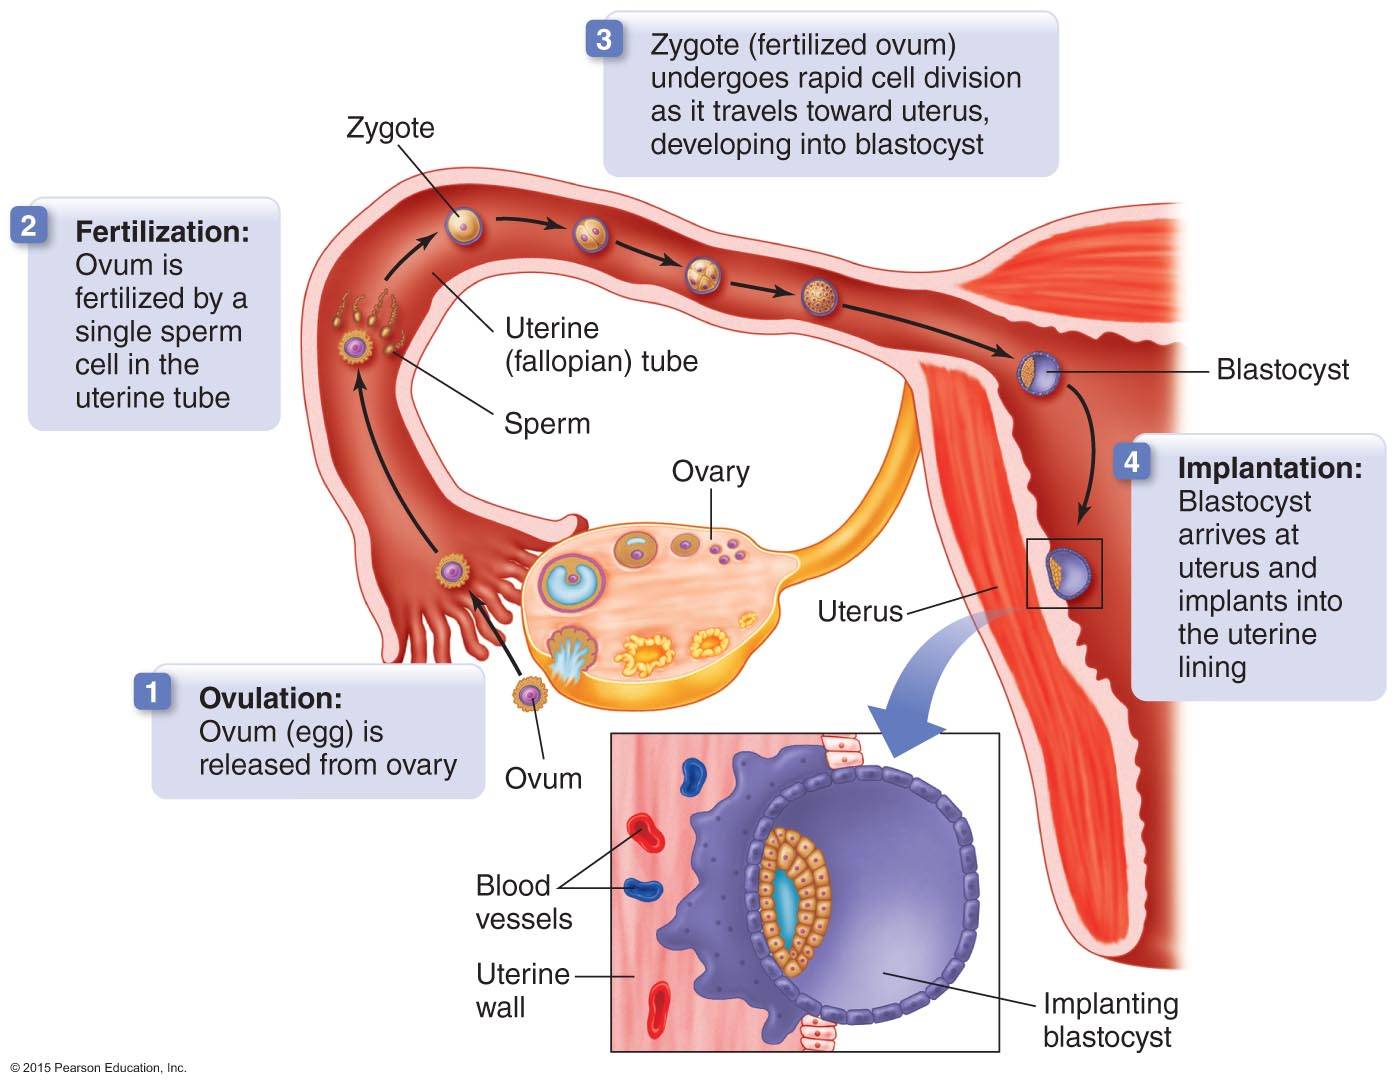
\includegraphics[width=\textwidth]{14_ovulation_conception_implantation}
	\caption{Ovulation, Conception, and Implantation}
	\label{fig:ovulation-conception-implantation}
\end{figure}

\begin{figure}[H]
	\centering
	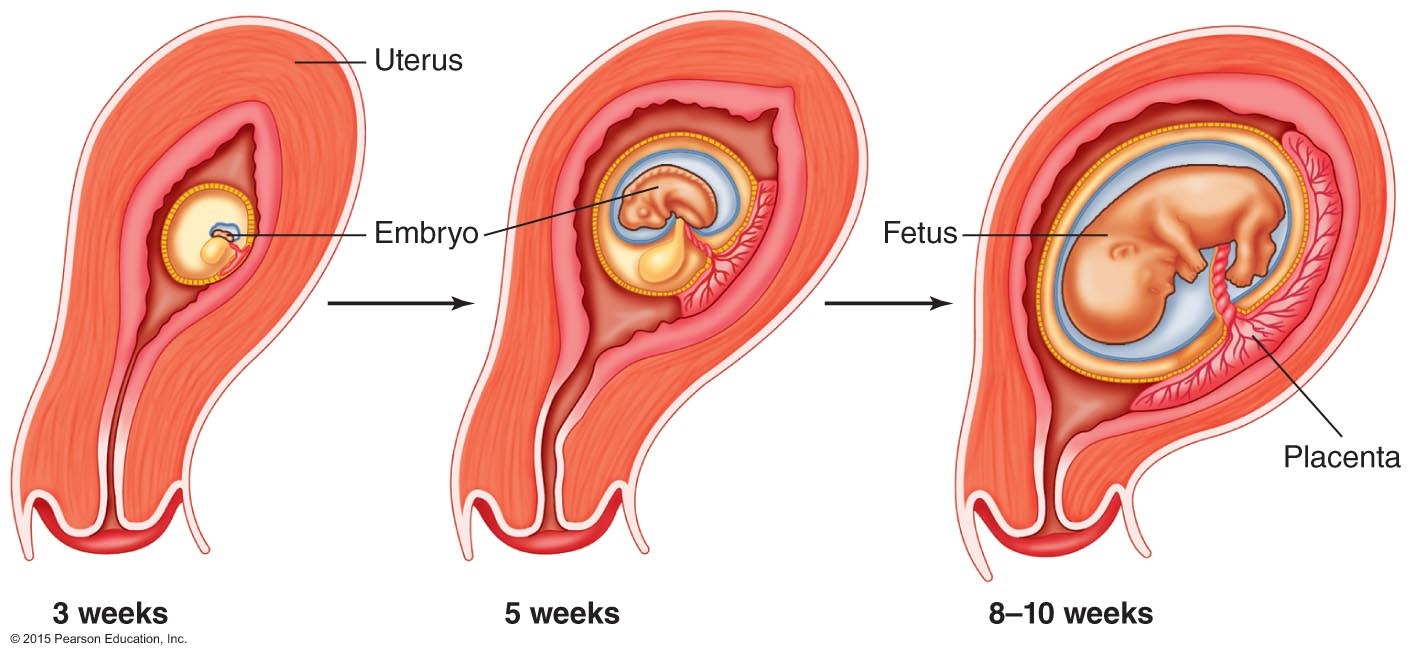
\includegraphics[width=\textwidth]{14_the_first_10_weeks}
	\caption{The First 10 Weeks}
	\label{fig:the-first-10-weeks}
\end{figure}

\begin{figure}[H]
	\centering
	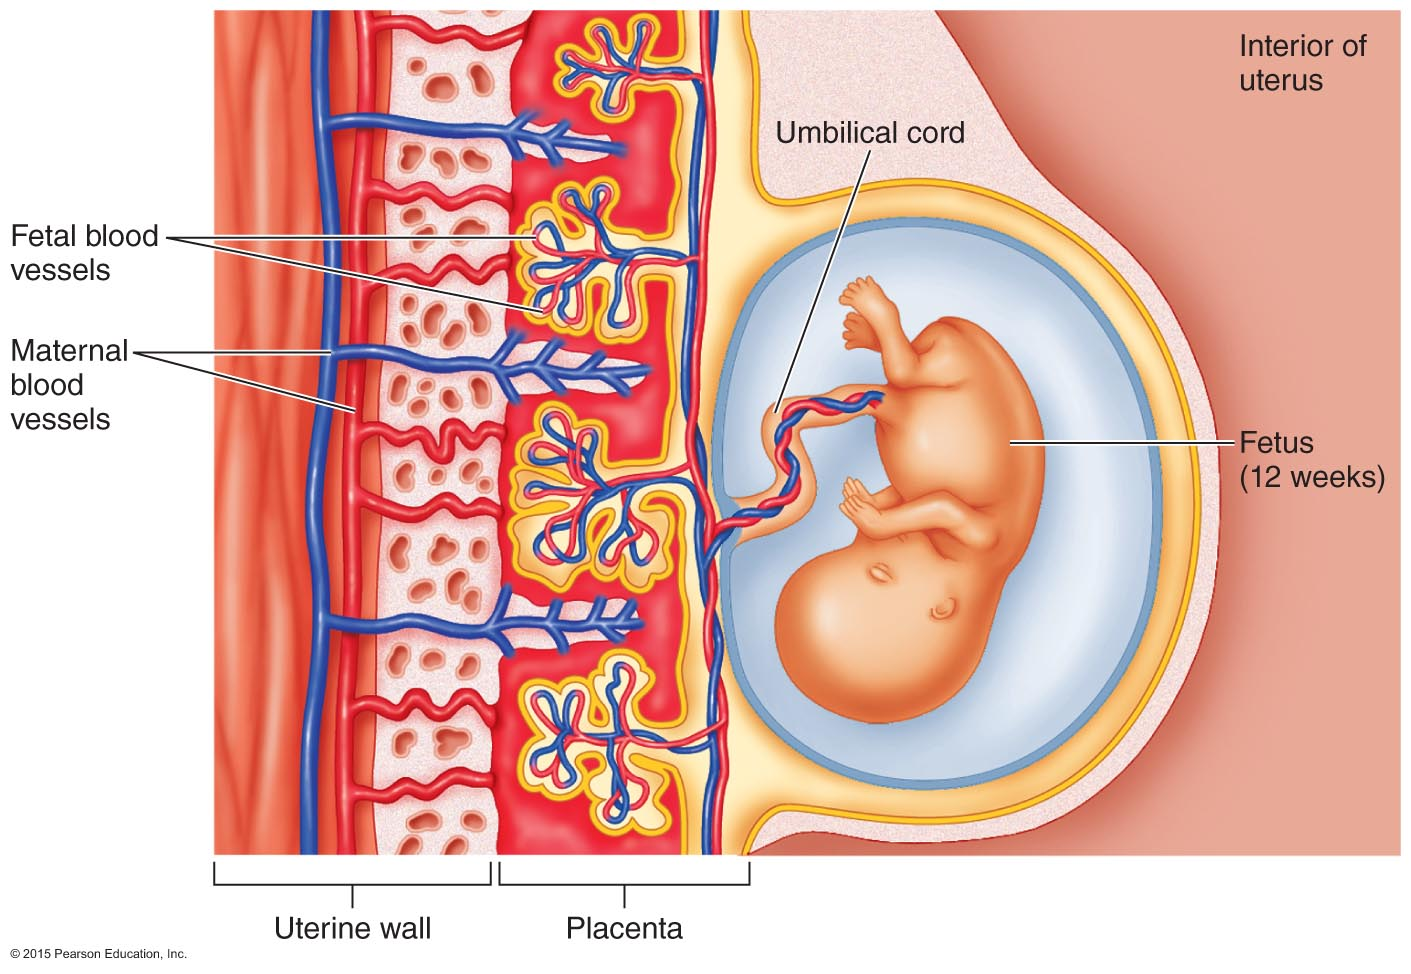
\includegraphics[width=\textwidth]{14_placental_development}
	\caption{Placental Development}
	\label{fig:placental-development}
\end{figure}

\subsection{Second trimester}\label{subsec:second-trimester}
\begin{itemize}
	\item Weeks 14--27
	\item Continued development of organ systems
	\item Growth from approximately 3 inches to over 1 foot long by the end of the second trimester
\end{itemize}

\subsection{Third trimester}\label{subsec:third-trimester}
\begin{itemize}
	\item Weeks 28 to birth
	\item Time of considerable growth
	\item Fetus gains three-quarters of its weight in this time
	\item Brain growth is also extensive
	\item Lungs become fully mature
	\item A balanced, adequate diet for the mother is essential during this time
\end{itemize}

\begin{figure}[H]
	\centering
	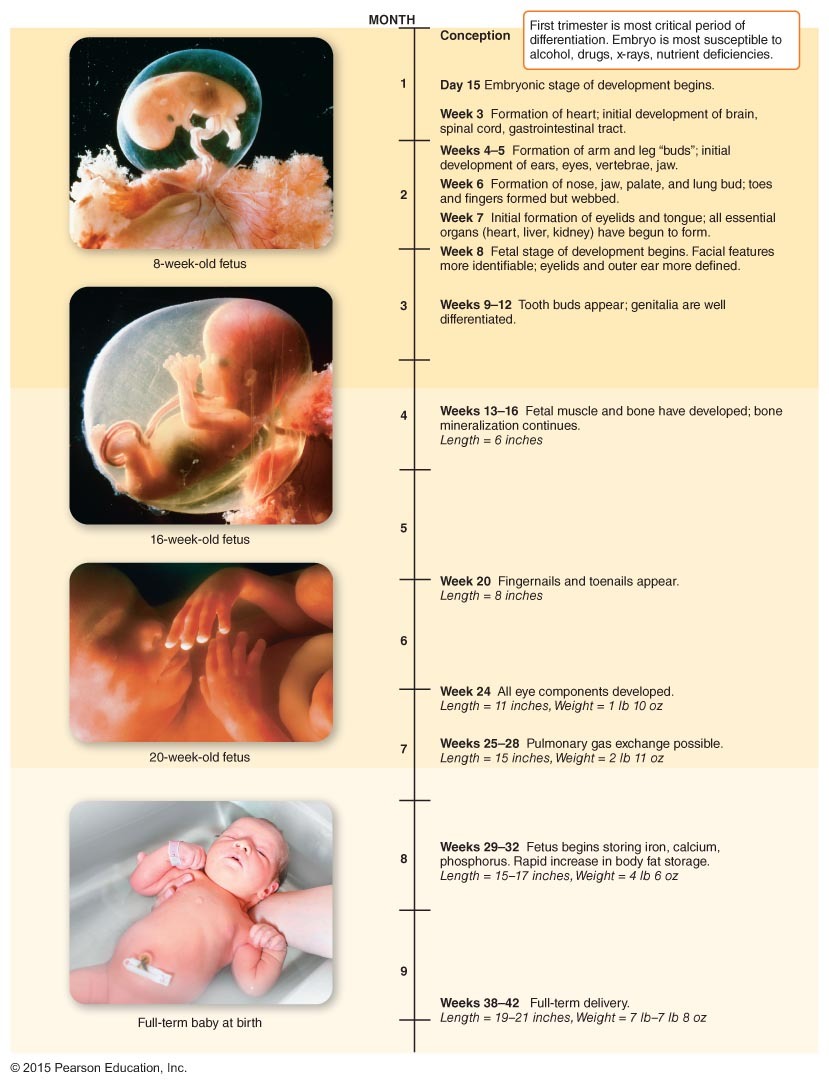
\includegraphics[width=\textwidth]{14_embryonic_and_fetal_development}
	\caption{Embryonic and Fetal Development}
	\label{fig:embryonic-and-fetal-development}
\end{figure}

\begin{itemize}
	\item An undernourished mother is more likely to give birth to a low-birth-weight baby
	\begin{itemize}
		\item \emph{Low birth weight:} describes any baby born weighing less than 5.5 pounds
		\item Increased risk of infections, learning disabilities, impaired physical development, and death in the first year
	\end{itemize}
\end{itemize}

\begin{figure}[H]
	\centering
	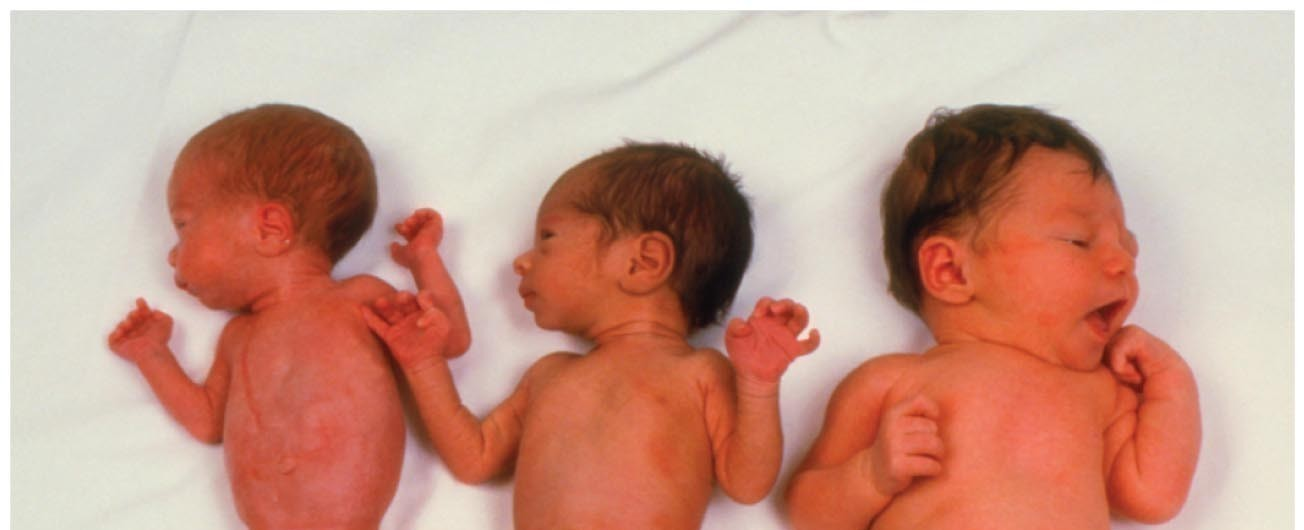
\includegraphics[width=\textwidth]{14_low_birth_weight_twins_and_healthy_infant}
	\caption{Low-Birth-Weight Twins and Healthy Infant}
	\label{fig:low-birth-weight-twins-and-healthy-infant}
\end{figure}

\begin{itemize}
	\item \emph{Preterm} babies are born before 38 weeks and may be low-birth-weight babies
	\item \emph{Small-for-gestational-age} babies are born at term but weigh less than would be expected for their gestational age
	\item Nutrition plays a major role in these conditions
\end{itemize}

\begin{itemize}
	\item Weight gain during pregnancy
	\begin{itemize}
		\item Women who do not gain enough weight are at risk of having a low-birth-weight baby
		\item Too much weight gain is also risky
		\item Women should not diet during pregnancy since this may deprive the fetus of critical nutrients
	\end{itemize}
\end{itemize}

\begin{figure}[H]
	\centering
	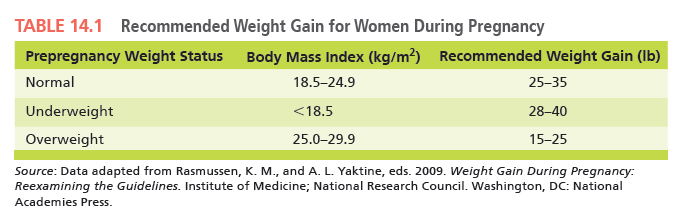
\includegraphics[width=\textwidth]{14_weight_gain_during_pregnancy}
	\caption{Weight Gain During Pregnancy}
	\label{fig:weight-gain-during-pregnancy}
\end{figure}

\begin{figure}[H]
	\centering
	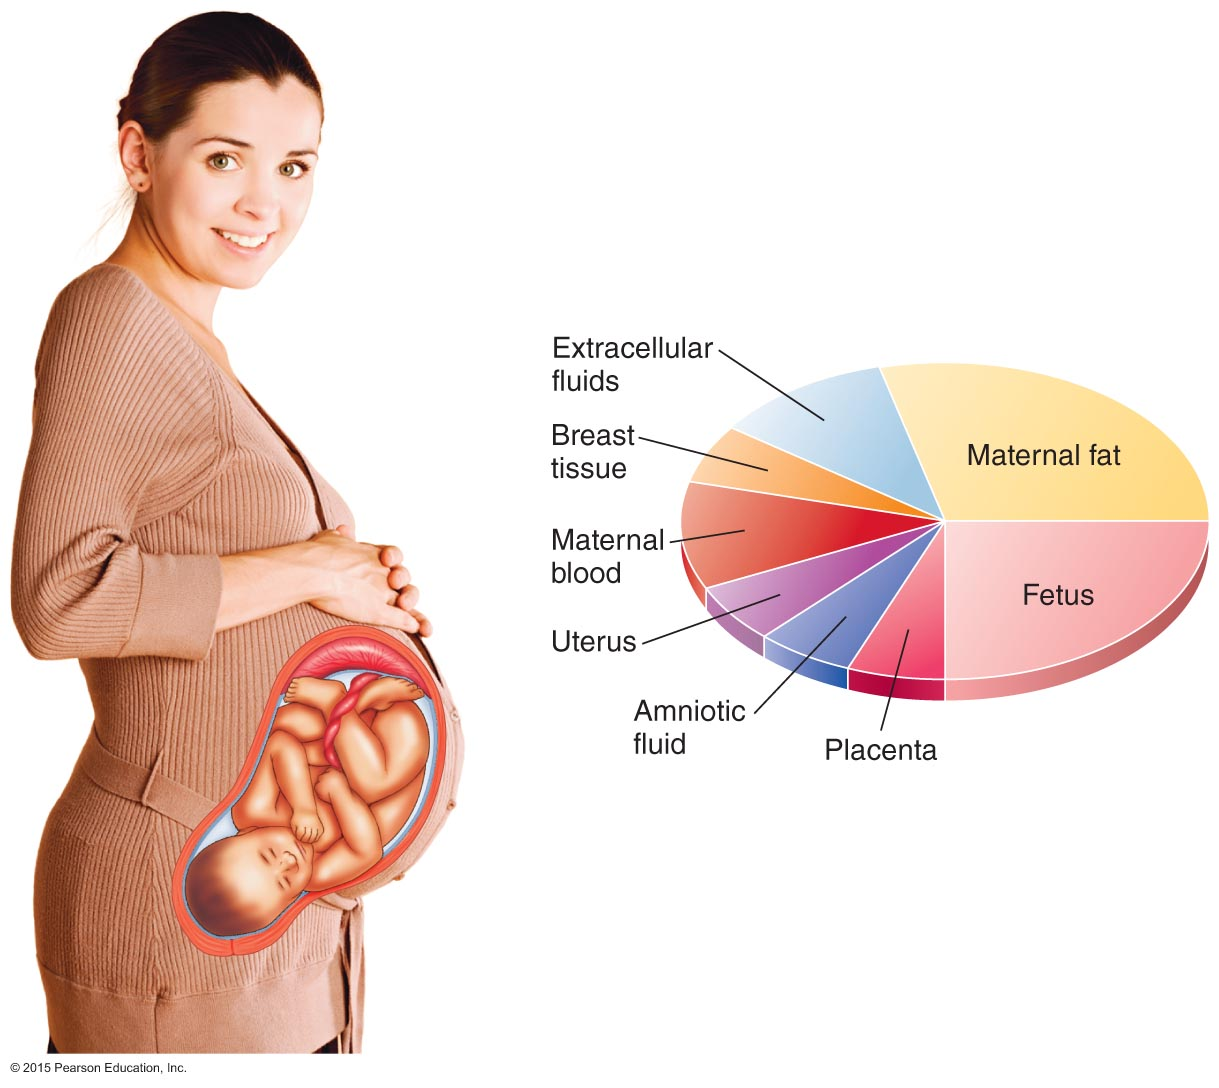
\includegraphics[width=\textwidth]{14_weight_gain_during_pregnancy_2}
	\caption{Weight Gain During Pregnancy (cont.))}
	\label{fig:weight-gain-during-pregnancy-cont}
\end{figure}

\begin{itemize}
	\item The requirement for nearly all nutrients increases during pregnancy
	\item Pregnant women must pay attention to their intake of:
	\begin{itemize}
		\item Macronutrients
		\item Micronutrients
		\item Fluids
	\end{itemize}
\end{itemize}

\section{Macronutrients}\label{sec:macronutrients}
\subsection{Energy}\label{subsec:energy}
\begin{itemize}
	\item An additional 300 to 450 kcal/day may be required in the second and third trimesters
	\item Nutrient-dense foods are essential in order to obtain sufficient nutrients
\end{itemize}

\subsection{Protein and carbohydrate}\label{subsec:protein-and-carbohydrate}
\begin{itemize}
	\item 1.1 g/day/kg body weight ($~\sim$additional 25 g/day) of protein
	\item At least 175 g/day of carbohydrates
\end{itemize}

\subsection{Fat}\label{subsec:fat}
\begin{itemize}
	\item The percentage of Calories obtained from fat should not change during pregnancy
	\item Limit saturated fat; avoid trans fats
	\item Consume rich sources of docosahexaenoic acid (DHA), an omega-3 polyunsaturated fatty acid
\end{itemize}

\section{Micronutrients}\label{sec:micronutrients}
\begin{table}[H]
	\centering
	\caption{The micronutrients that are most critical during pregnancy include}
	\label{tab:pregnancy-micronutrients}
	\begin{tabular}{l l}
		folate		& calcium\\
		vitamin $\mbox{B}_{12}$	& iron\\
		vitamin C	& zinc\\
		vitamin A	& sodium\\
		vitamin D	& iodine\\
	\end{tabular}
\end{table}

\begin{figure}[H]
	\centering
	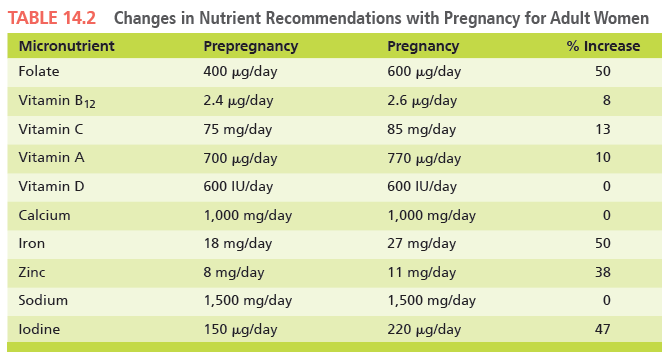
\includegraphics[width=\textwidth]{14_nutrient_recommendations}
	\caption{Nutrient Recommendations}
	\label{fig:nutrient-recommendations}
\end{figure}

\subsection{Folate}\label{subsec:folate}
\begin{itemize}
	\item Required for cell division
	\item Critical in the first 28 days for development of the \emph{neural tube}, which becomes the brain and spinal cord
	\item 400 $\mu$g/day for sexually active women
	\item 600 $\mu$g/day for pregnant women
	\item Deficiency is associated with \emph{anencephaly} and \emph{spina bifida}
\end{itemize}

\begin{figure}[H]
	\centering
	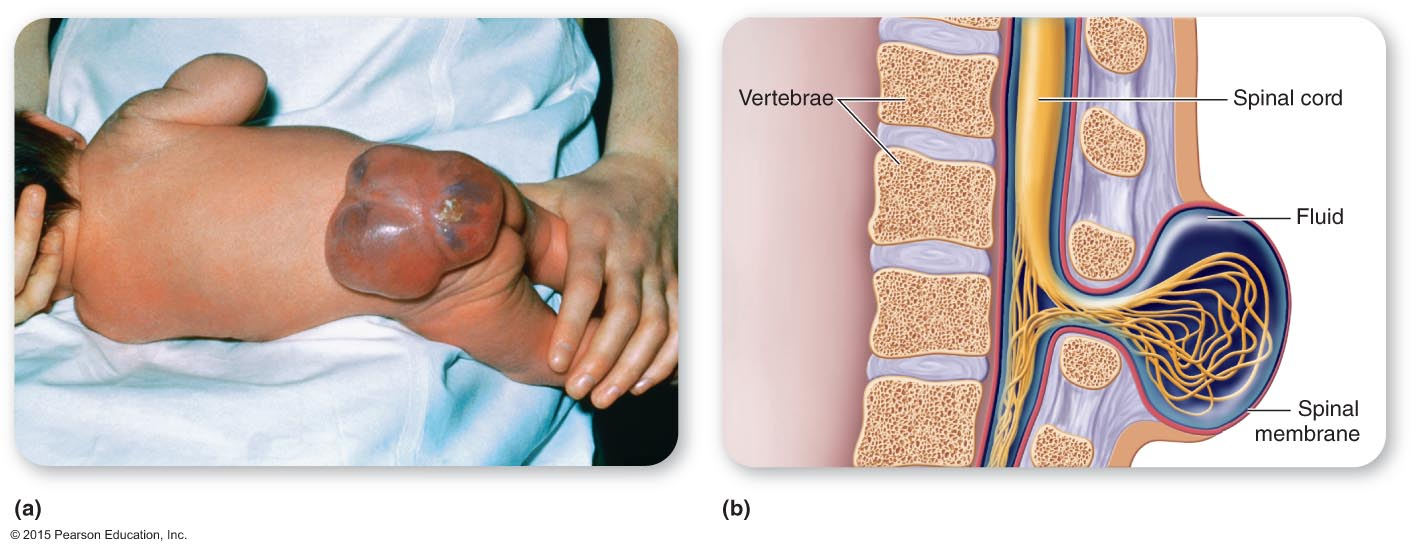
\includegraphics[width=\textwidth]{14_spina_bifida}
	\caption{Spina Bifida}
	\label{fig:spina-bifida}
\end{figure}

\subsection{Vitamin $\mbox{B}_{12}$}\label{subsec:vitamin-b12}
\begin{itemize}
	\item Regenerates the active form of folate
	\item 2.6 $\mu$g/day during pregnancy
\end{itemize}

\subsection{Vitamin C}\label{subsec:vitamin-c}
\begin{itemize}
	\item Production of collagen (connective tissue)
	\item 85 mg/day during pregnancy
	\item Deficiency results in elevated risk of preterm births and preeclampsia
\end{itemize}

\subsection{Vitamin A}\label{subsec:vitamin-a}
\begin{itemize}
	\item Needs increase by 10\% in pregnancy
	\item 770 $\mu$g/day
	\item Excess vitamin A can cause fetal abnormalities
	\item Supplementation is not recommended due to toxicity risk
	\item Beta-carotene (provitamin A) is not associated with birth defects
\end{itemize}

\subsection{Vitamin D}\label{subsec:vitamin-d}
\begin{itemize}
	\item Adequate intake (AI) does not increase during pregnancy
	\item Excessive vitamin D can cause developmental disabilities in newborns
	\item If exposure to sunlight is limited or milk consumption is low, supplementation is advised
	\item Prenatal vitamin supplements contain 10 $\mu$g/dose
\end{itemize}

\subsection{Calcium}\label{subsec:calcium}
\begin{itemize}
	\item 1,000 mg/day, same as for non-pregnant women
	\item Calcium absorption is more efficient during pregnancy
\end{itemize}

\subsection{Iron}\label{subsec:iron}
\begin{itemize}
	\item Increased need for red blood cells increases the need for iron by 50–80\% (27 mg/day)
	\item Fetal need for iron increases in the third trimester
	\item Iron stores of mother are depleted to support needs of the fetus
	\item Iron-deficiency anemia is common during pregnancy
\end{itemize}

\subsection{Zinc}\label{subsec:zinc}
\begin{itemize}
	\item Critical for making proteins, DNA, and RNA
	\item Need increases 38\% during pregnancy (11 mg/day)
\end{itemize}

\subsection{Sodium}\label{subsec:sodium}
\begin{itemize}
	\item 1,500 mg/day, same as for non-pregnant women
\end{itemize}

\subsection{Iodine}\label{subsec:iodine}
\begin{itemize}
	\item Need for iodine increases significantly
	\item 220 $\mu$g/day can be obtained from iodized salt
\end{itemize}

\section{Fluids During Pregnancy}\label{sec:fluids-during-pregnancy}
\begin{itemize}
	\item The amount of fluids needed increases to 3 liters per day
	\begin{itemize}
		\item Increase in maternal blood volume
		\item Body temperature regulation
		\item Production of \emph{amniotic fluid} to protect and cushion the fetus
		\item Combat fluid retention and constipation
		\item Reduce risk of \emph{urinary tract infections}
	\end{itemize}
\end{itemize}

\subsection{Nutrition-Related Concerns}\label{subsec:nutrition-related-concerns}
\begin{itemize}
	\item Nutrition-related problems during pregnancy can include
	\begin{itemize}
		\item Morning sickness
		\item Food and nonfood cravings and aversions
		\item Gastroesophageal reflux (GER)/heartburn
		\item Constipation
		\item Gestational diabetes
		\item Preeclampsia (maternal blood pressure increase)
	\end{itemize}
\end{itemize}

\section{Morning Sickness}\label{sec:morning-sickness}
\begin{itemize}
	\item \definition{Morning sickness}{nausea and vomiting associated with pregnancy}
	\begin{itemize}
		\item Can occur at any time; often lasts all day
		\item May begin after the first missed period and can last 12 to 16 weeks
		\item Can be severe enough to require hospitalization
		\item No cure, but symptoms can be reduced
	\end{itemize}
\end{itemize}

\section{Cravings and Aversions}\label{sec:cravings-and-aversions}
\begin{itemize}
	\item Most women crave a certain type of food (sweet, salty) rather than a specific food
	\begin{itemize}
		\item Little evidence supports the idea that cravings indicate a deficiency
		\item Due to hormonal fluctuations, physiologic changes, or familial or cultural roots
		\item \definition{Pica}{craving a nonfood item (ice, clay, laundry starch)}
		\item Food aversions are common but not universal among pregnant women
	\end{itemize}
\end{itemize}

\subsection{Gastroesophageal Reflux (GER)}\label{subsec:gastroesophageal-reflux-(ger)}
\begin{itemize}
	\item Gastroesophageal reflux (GER) is common during pregnancy
	\item Tips to help minimize it include
	\begin{itemize}
		\item Avoid excessive weight gain
		\item Chew food slowly
		\item Wait for 1 hour after eating before lying down
		\item Sleep with your head elevated
	\end{itemize}
\end{itemize}

\section{Constipation}\label{sec:constipation}
\begin{itemize}
	\item Pregnancy hormones that cause smooth muscles to relax also slow the movement of material through the large intestine
	\item Reduce constipation by consuming 25–35 g/day of fiber and plenty of fluids, and remaining physically active
\end{itemize}

\section{Gestational Diabetes}\label{sec:gestational-diabetes}
\begin{itemize}
	\item \definition{Gestational diabetes}{insufficient insulin production or insulin resistance that increases blood glucose levels during pregnancy}
	\begin{itemize}
		\item Affects as many as 10\% of U.S.\@ pregnancies
		\item Condition resolves after birth occurs
		\item Risk of delivering a large baby
		\item Gestational diabetes increases a woman’s risk of developing type 2 diabetes
	\end{itemize}
\end{itemize}

\section{Gestational Hypertension}\label{sec:gestational-hypertension}
\begin{itemize}
	\item \definition{Preeclampsia}{pregnancy-induced hypertension}
	\begin{itemize}
		\item Affects up to 10\% of U.S. pregnancies
		\item Can be fatal if left untreated
		\item Deficiencies in vitamin C, vitamin E, and magnesium increase the risk
		\item Treatment focuses on managing blood pressure and often includes bed rest
		\item The only cure is childbirth
	\end{itemize}
\end{itemize}

\section{Foodborne Illness}\label{sec:foodborne-illness}
\begin{itemize}
	\item Pregnancy alters a woman’s immune system leaving them more vulnerable to infectious diseases including foodborne illnesses
	\begin{itemize}
		\item Listeriosis: a serious and sometimes fatal illness caused my listeria monocytogenes
		\item Third leading cause of death by foodborne illness
		\item Severe infections of listeria can lead to premature birth or miscarriage
	\end{itemize}
\end{itemize}

\section{Food Safety}\label{sec:food-safety}
\begin{itemize}
	\item Pregnant women should avoid consuming
	\begin{itemize}
		\item Unpasteurized milk, raw or partially cooked eggs, raw or undercooked meat/fish/poultry, unpasteurized juices, and raw sprouts
		\item Large fish such as shark, swordfish, and king mackerel, along with canned albacore tuna
		\item Soft cheeses unless the label specifically states the product is made with pasteurized milk
	\end{itemize}
\end{itemize}

\begin{figure}[H]
	\centering
	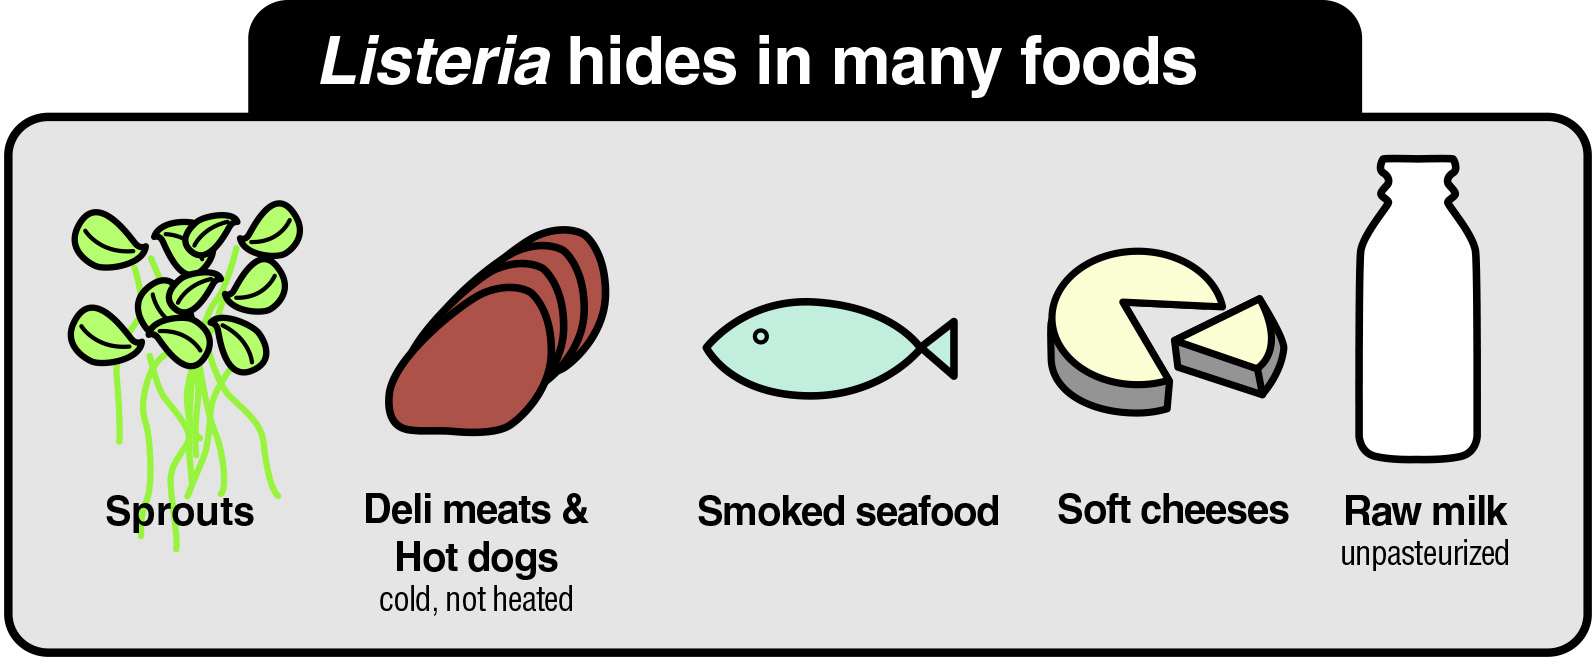
\includegraphics[width=\textwidth]{14_foodborne_illness}
	\caption{Foodborne Illness}
	\label{fig:foodborne-illness}
\end{figure}

\section{Nutrition-Related Concerns}\label{sec:nutrition-related-concerns}
\begin{itemize}
	\item Adolescent pregnancy
	\item Vegetarianism
	\item Exercise
	\item Caffeine consumption
	\item Alcohol consumption
	\item Smoking
	\item Illegal drug use
	\item Food safety
\end{itemize}

\section{Adolescent Pregnancy}\label{sec:adolescent-pregnancy}
\begin{itemize}
	\item Nutritional needs of pregnant adolescents are higher than those of adult women
	\item Adolescent bodies are still growing and changing, adding to the nutritional needs of pregnancy
	\item 24 births for every 1,000 adolescents; currently the lowest adolescent pregnancy rate in 60 years
\end{itemize}

\section{Vegetarianism}\label{sec:vegetarianism}
\begin{itemize}
	\item A vegetarian consuming eggs and dairy products has the same nutritional concerns as a nonvegetarian
	\begin{table}[H]
		\centering
		\caption{A complete vegetarian (vegan) must carefully monitor the intake of}
		\label{tab:pregnant-vegetarian-intake}
		\begin{tabular}{l l}
			vitamin D & calcium\\
			vitamin $\mbox{B}_{6}$ & iron\\
			vitamin $\mbox{B}_{12}$ & zinc\\
		\end{tabular}
	\end{table}
\end{itemize}

\section{Exercise During Pregnancy}\label{sec:exercise-during-pregnancy}
\begin{itemize}
	\item Reduces risk of gestational diabetes and preeclampsia
	\item Helps prevent excessive prenatal weight and body fat gain
	\item Improves mood, energy level, sleep patterns
	\item Enhances posture and balance
	\item Improves muscle tone, strength, and endurance
	\item Reduces lower back pain and shortens the duration of active labor
	\item Reduces risk of preterm birth and large-for-gestational age infants
\end{itemize}

\section{Consumption of Caffeine}\label{sec:consumption-of-caffeine}
\begin{itemize}
	\item Caffeine is a stimulant that crosses the placenta and reaches the fetus
	\item 200–300 mg of caffeine per day very likely will cause no harm
	\item Some studies have linked 100 mg per day intakes to an increased risk of miscarriage, stillbirth, preterm birth, and decreased birth weight
\end{itemize}

\section{Consumption of Alcohol}\label{sec:consumption-of-alcohol}
\begin{itemize}
	\item Alcohol is a known \hyperref[dfn:teratogen]{teratogen} that crosses the placenta and is associated with various birth defects, delivery complications, sudden infant death syndrome, and increased risk of miscarriage
	\item \hyperref[dfn:fas]{Fetal alcohol syndrome (FAS)}: variety of characteristics associated with prenatal exposure to high quantities of alcohol
	\begin{itemize}
		\item Malformations of face, limbs, heart, and nervous system
		\item Many developmental disabilities
	\end{itemize}
\end{itemize}

\section{Smoking and Drug Use}\label{sec:smoking-and-drug-use}
\begin{itemize}
	\item Maternal smoking exposes the fetus to toxins
	\begin{itemize}
		\item Smoke contains lead, cadmium, cyanide, nicotine, and carbon monoxide
		\item Fetal blood flow is reduced
		\item Increased risk of miscarriage, stillbirth, placental abnormalities, preterm delivery, and low birth weight
	\end{itemize}
	\item Most drugs pass through the placenta into fetal blood
	\begin{itemize}
		\item Newborns suffer withdrawal symptoms
	\end{itemize}
\end{itemize}

\section{Breastfeeding}\label{sec:breastfeeding}
\begin{itemize}
	\item \definition{Lactation}{production of breast milk}
	\begin{itemize}
		\item \definition{Prolactin}{hormone responsible for the synthesis of milk}
		\begin{itemize}
			\item Produced toward the end of pregnancy
			\item Suppressed by estrogen and progesterone until childbirth
		\end{itemize}
	\end{itemize}
	\item \definition{Colostrum}{first milk produced (from birth up to 3 days after); rich in proteins, antibodies, vitamins, and minerals}
	\begin{itemize}
		\item \definition{Oxytocin}{hormone responsible for milk let-down}
	\end{itemize}
\end{itemize}

\begin{figure}[H]
	\centering
	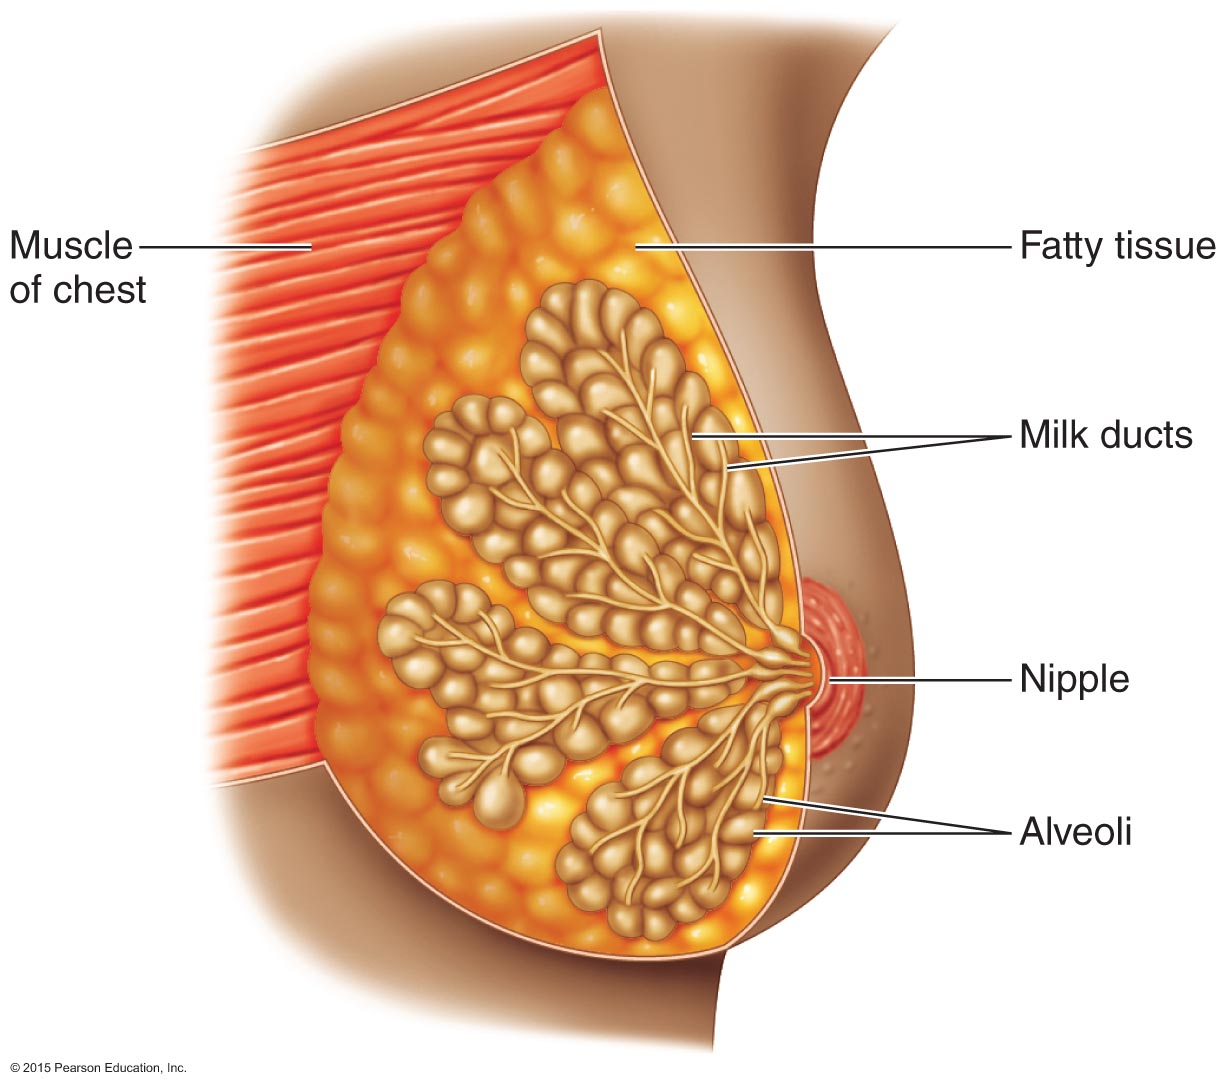
\includegraphics[width=\textwidth]{14_anatomy_of_the_breast}
	\caption{Anatomy of the Breast}
	\label{fig:anatomy-of-the-breast}
\end{figure}

\begin{figure}[H]
	\centering
	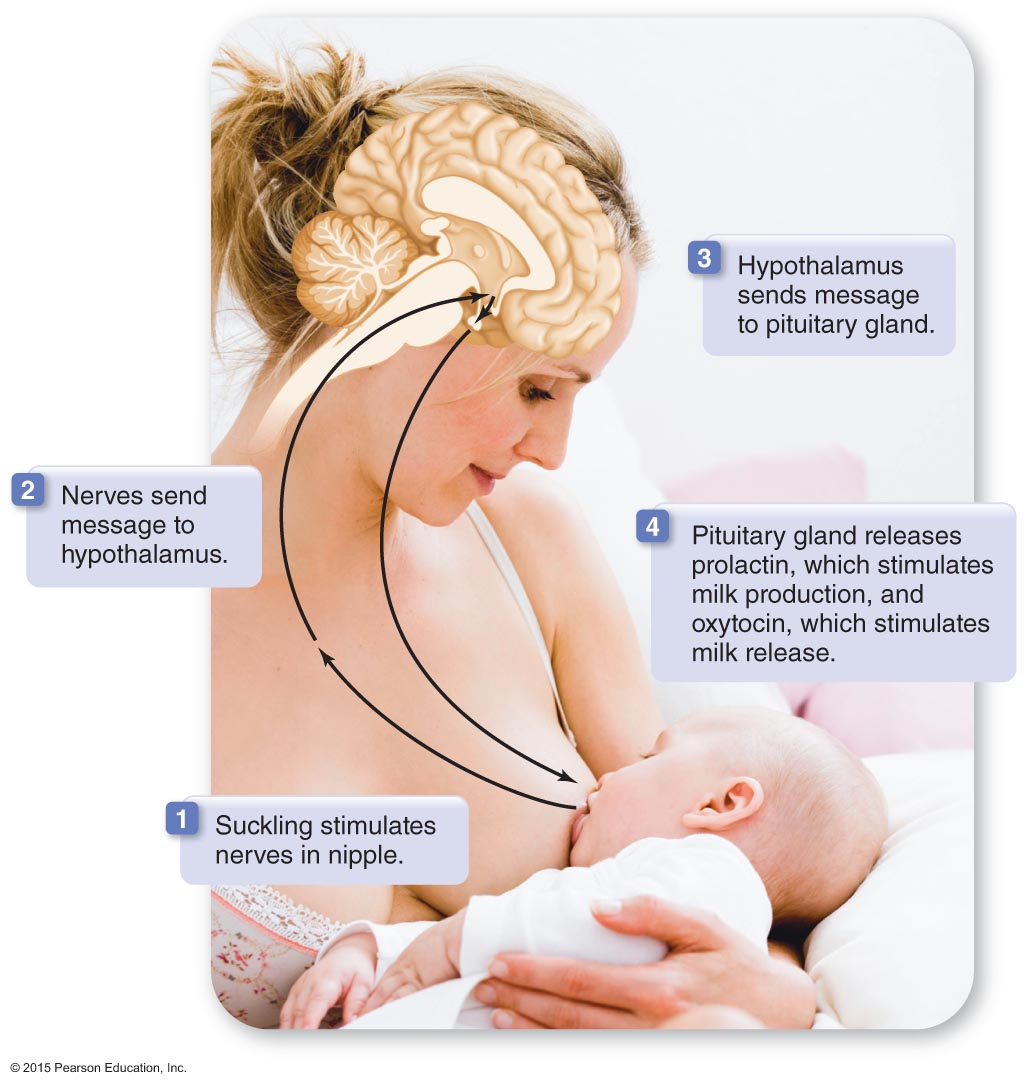
\includegraphics[width=\textwidth]{14_milk_and_mother_child_interaction}
	\caption{Milk and Mother--Child Interaction}
	\label{fig:milk-and-mother-child-interaction}
\end{figure}

\begin{itemize}
	\item Milk production requires 700–800 kcal/day
	\item Lactating women should consume 330 kcal/day above their prepregnancy needs the first 6 months, 400 kcal/day the second 6 months
	\item This allows a woman to gradually lose weight (1–4 pounds per month)
	\item 15–20 g of protein and 80 g of carbohydrate required per day above prepregnancy needs
	\item Fluid and many micronutrient needs are increased
\end{itemize}

\begin{figure}[H]
	\centering
	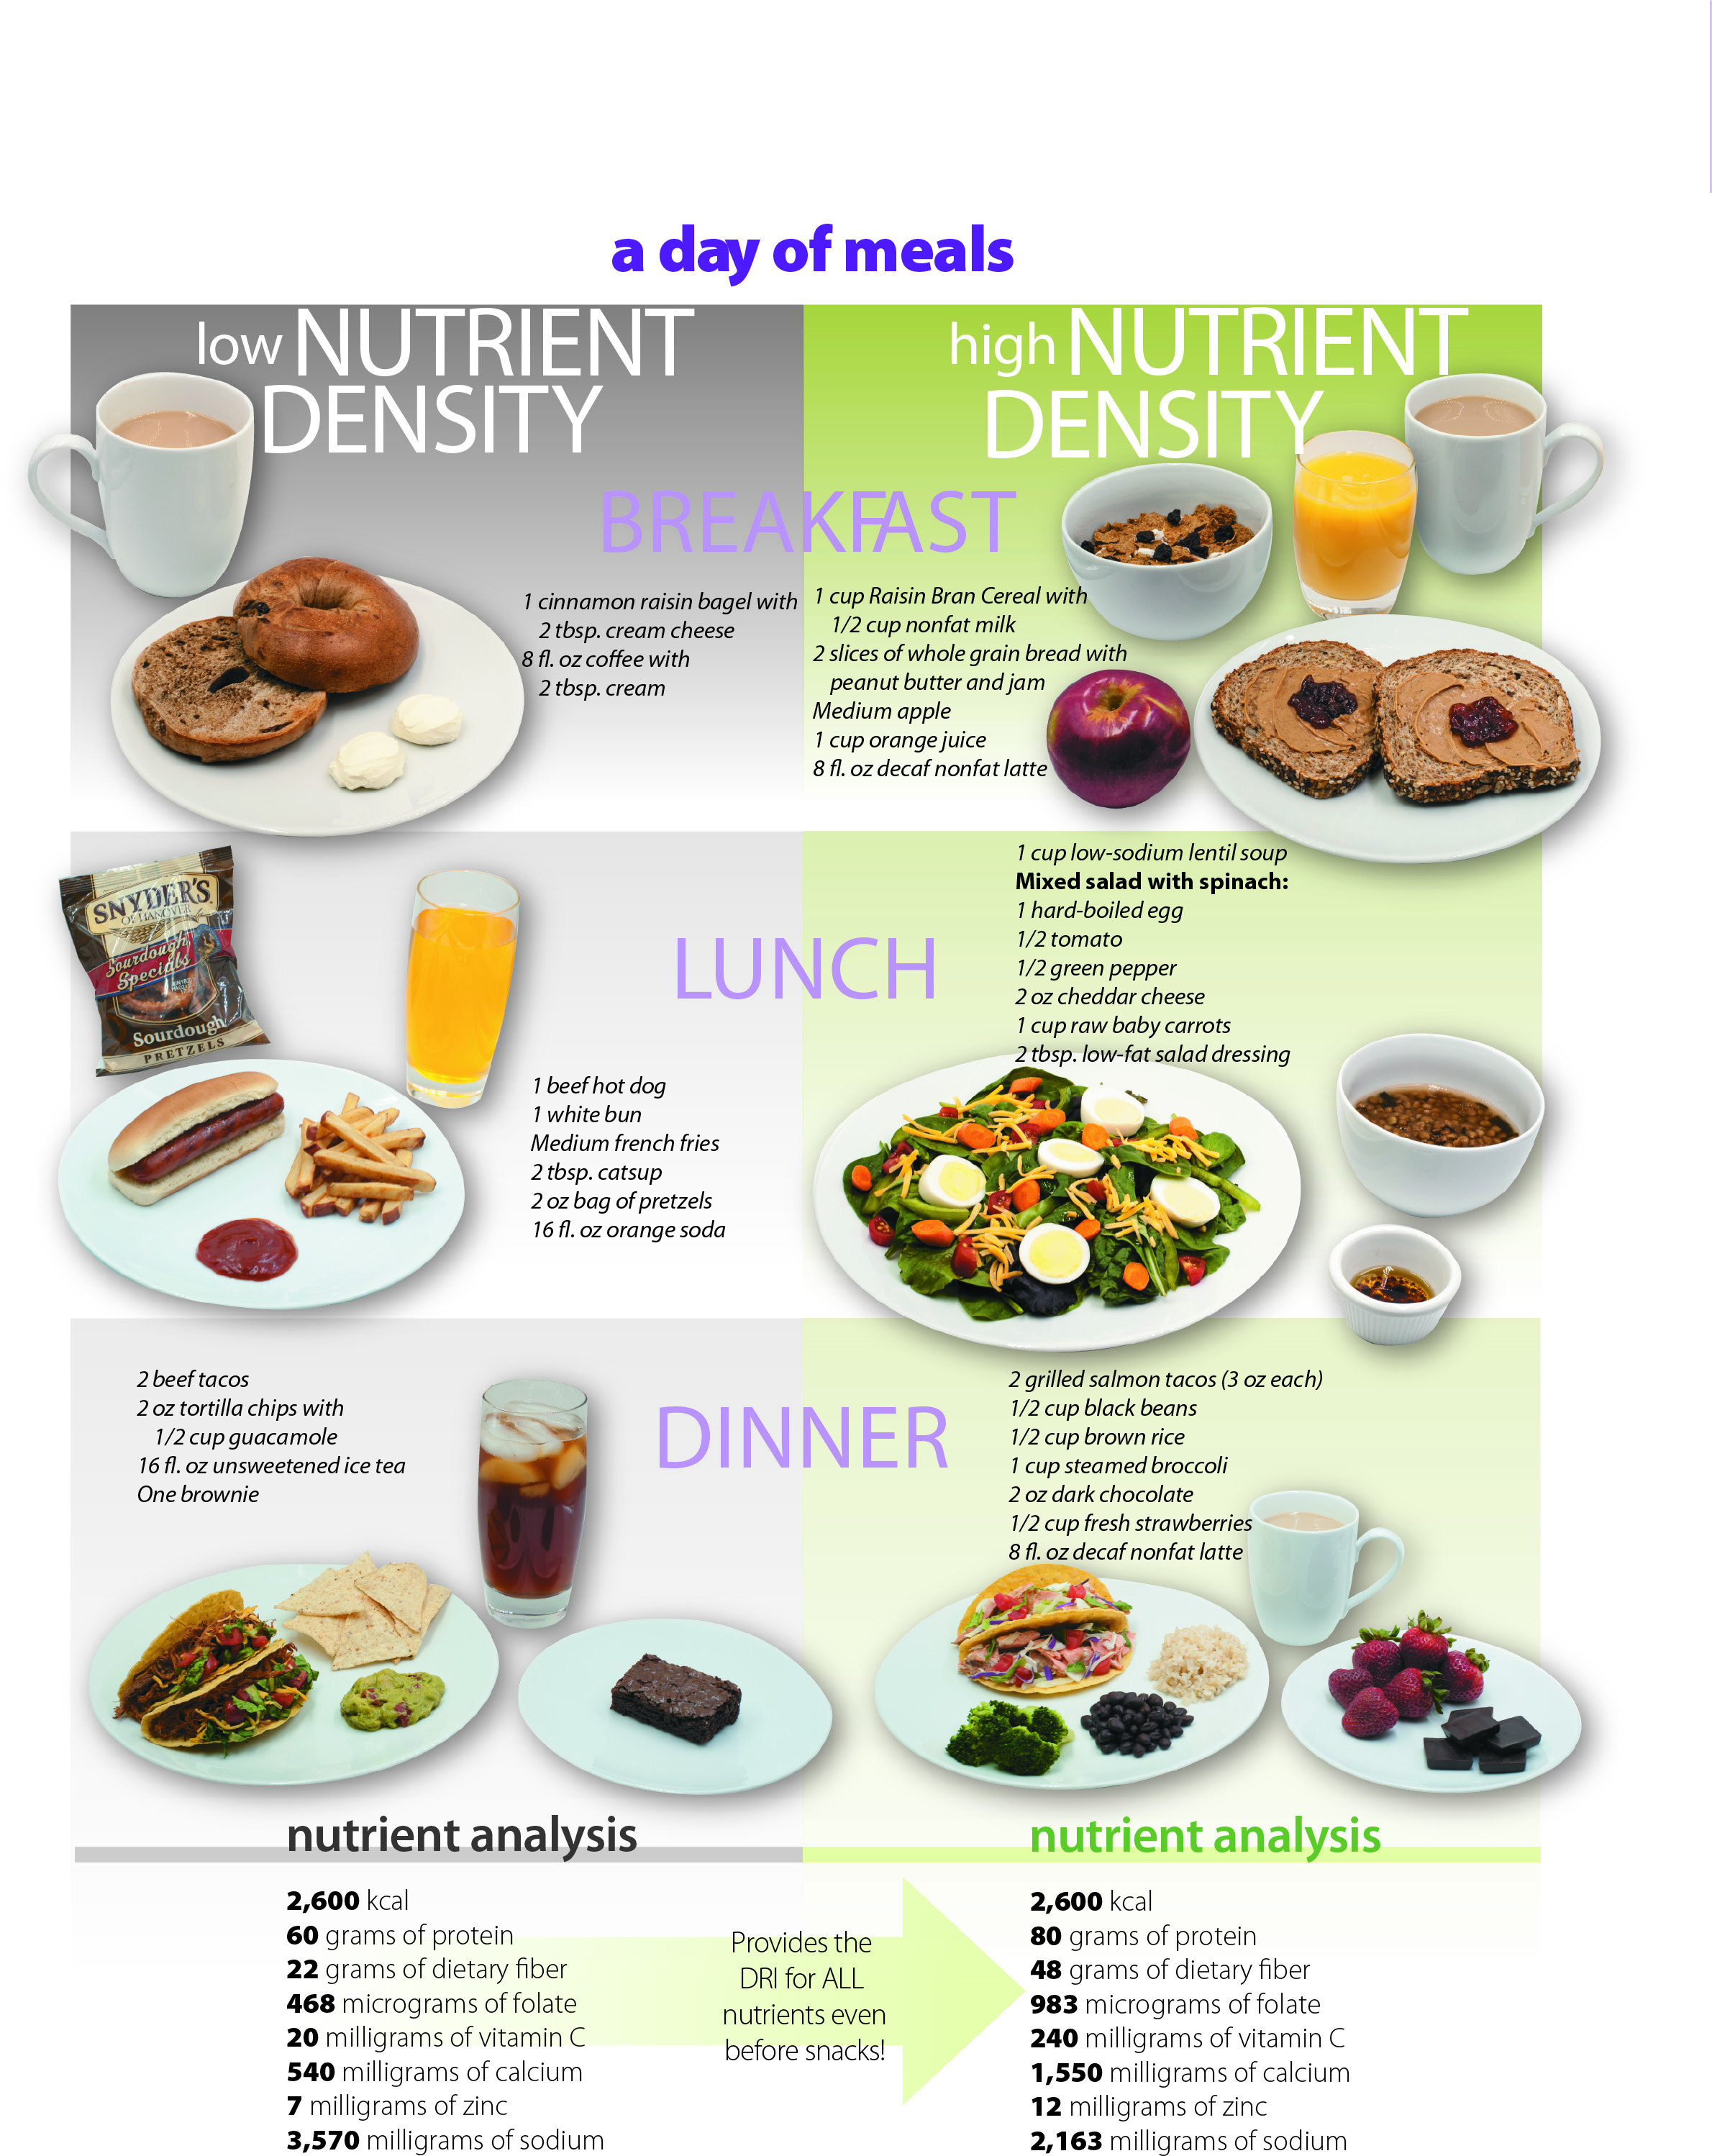
\includegraphics[width=\textwidth]{14_breastfeeding_2}
	\caption{Breastfeeding (cont.)}
	\label{fig:breastfeeding-2}
\end{figure}

\subsection{The Benefits of Breastfeeding}\label{subsec:the-benefits-of-breastfeeding}
\begin{itemize}
	\item High-quality nutrition
	\item Protection from infections, allergies, and residues
	\item Assists the mother in weight loss
	\item Suppresses ovulation
	\item Provides an opportunity for bonding
	\item Convenience and cost efficient
\end{itemize}

\begin{itemize}
	\item Nutritional quality of breast milk
	\begin{itemize}
		\item The main protein, lactalbumin, is easily digested
		\item Primary carbohydrate is lactose
		\item Rich source of readily absorbed calcium and magnesium
	\end{itemize}
	\item Composition of milk changes during a feeding
	\begin{description}
		\item[Foremilk:] watery and low in fat
		\item[Hindmilk:] very high in fat
	\end{description}
	\item It is important to let infant suckle for at least 20 minutes
\end{itemize}

\section{Challenges Associated with Breastfeeding}\label{sec:challenges-associated-with-breastfeeding}
\begin{itemize}
	\item Many harmful substances are passed into breast milk, including
	\begin{itemize}
		\item Illegal drugs, caffeine, nicotine, and prescription and over-the-counter medications
	\end{itemize}
	\item HIV is passed through breast milk
	\item Conflicts with mother’s employment
	\item Social concerns
\end{itemize}

\section{Infant Nutrition}\label{sec:infant-nutrition}
\begin{itemize}
	\item Optimal nutrition is critical in the first year
	\begin{itemize}
		\item High energy needs, 40–50 kcal/lb/day
		\item 40–50\% of energy should come from fat
		\item Iron, vitamin D, zinc, fluoride, and iodide needs are a concern
		\item The nervous system continues to develop
		\item Infants typically grow 10 inches in length and triple their weight in the first year
	\end{itemize}
	\item Infants’ nutritional needs are unique
	\begin{itemize}
		\item Their energy needs are high to support rapid growth
		\item Their digestive tracts and kidneys are still immature
		\item They are small in size
	\end{itemize}
\end{itemize}

\begin{figure}[H]
	\centering
	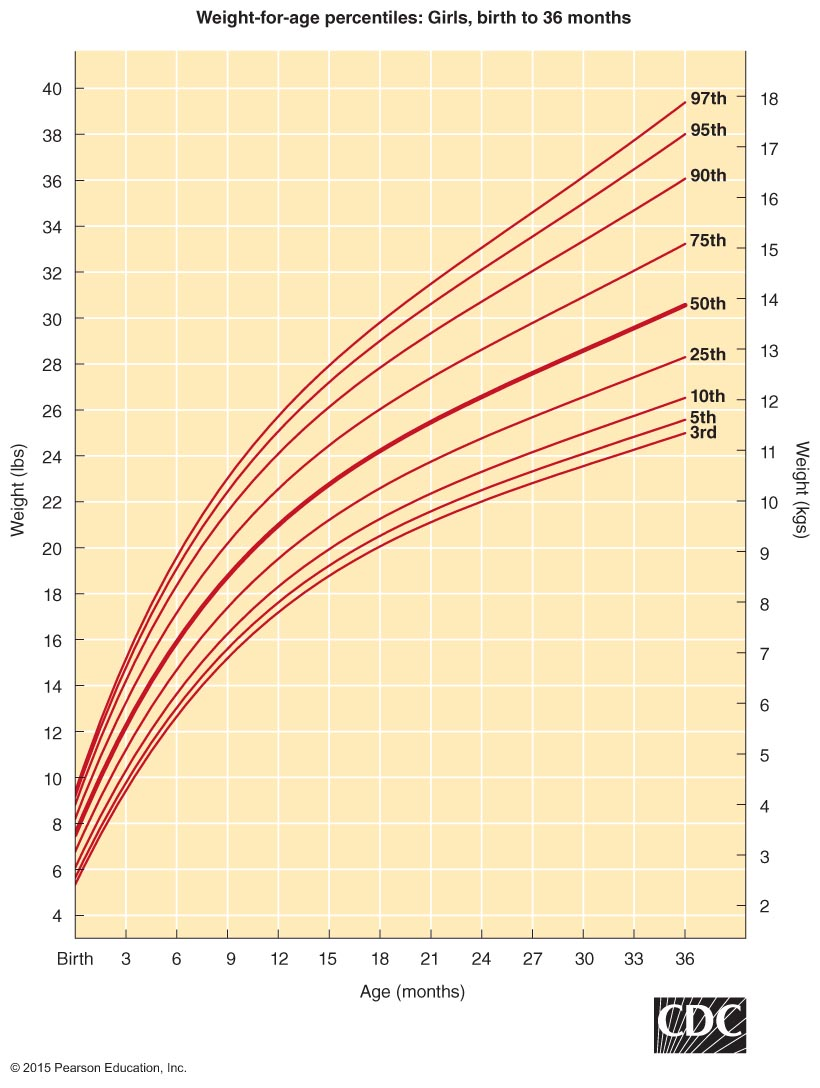
\includegraphics[width=\textwidth]{14_weight_to_age_growth_chart}
	\caption{Weight-to-Age Growth Chart}
	\label{fig:weight-to-age-growth-chart}
\end{figure}

\subsection{Infant Nutrient Needs}\label{subsec:infant-nutrient-needs}
\begin{itemize}
	\item 40–50 kcals per pound of body weight per day
	\begin{itemize}
		\item Approximately 600–650 kcals per day at around 6 months of age
		\item Breastmilk and commercial formulas are energy and nutrient dense to meet these demands
	\end{itemize}
\end{itemize}

% End Infant Nutrient needs

\begin{itemize}
	\item Breast milk or formula should be supplemented with solid food beginning at 4 to 6 months
	\item 40–50\% of energy needs should be consumed from fat during the first year of life
	\item No more than 20\% of an infant’s daily energy needs should be consumed from protein
\end{itemize}

\section{Supplements for Infants?}\label{sec:supplements-for-infants?}
\begin{itemize}
	\item Several micronutrients may need supplementation
	\begin{itemize}
		\item Vitamin D because of limited exposure to sunlight
		\item Iron--stores are depleted by the sixth month
		\item Fluoride for tooth development
		\item Vitamin $\mbox{B}_{12}$ if the mother is a vegan
		\item Water is generally not required unless loss is excessive (diarrhea, vomiting, fever, hot weather)
	\end{itemize}
	\item Care must be taken to prevent oversupplementation
\end{itemize}

\section{Formulas}\label{sec:formulas}
\begin{itemize}
	\item Very tightly regulated by federal government
	\begin{itemize}
		\item Minimum and maximum standards for 29 nutrients
		\item Protein source: casein or whey from cow’s milk
		\item Carbohydrate source: lactose and sucrose
		\item Fat source: vegetable oils or microbiologically produced lipids
	\end{itemize}
	\item Specialized formulas are available: soy-based, predigested, others for certain medical conditions
\end{itemize}

\begin{figure}[H]
	\centering
	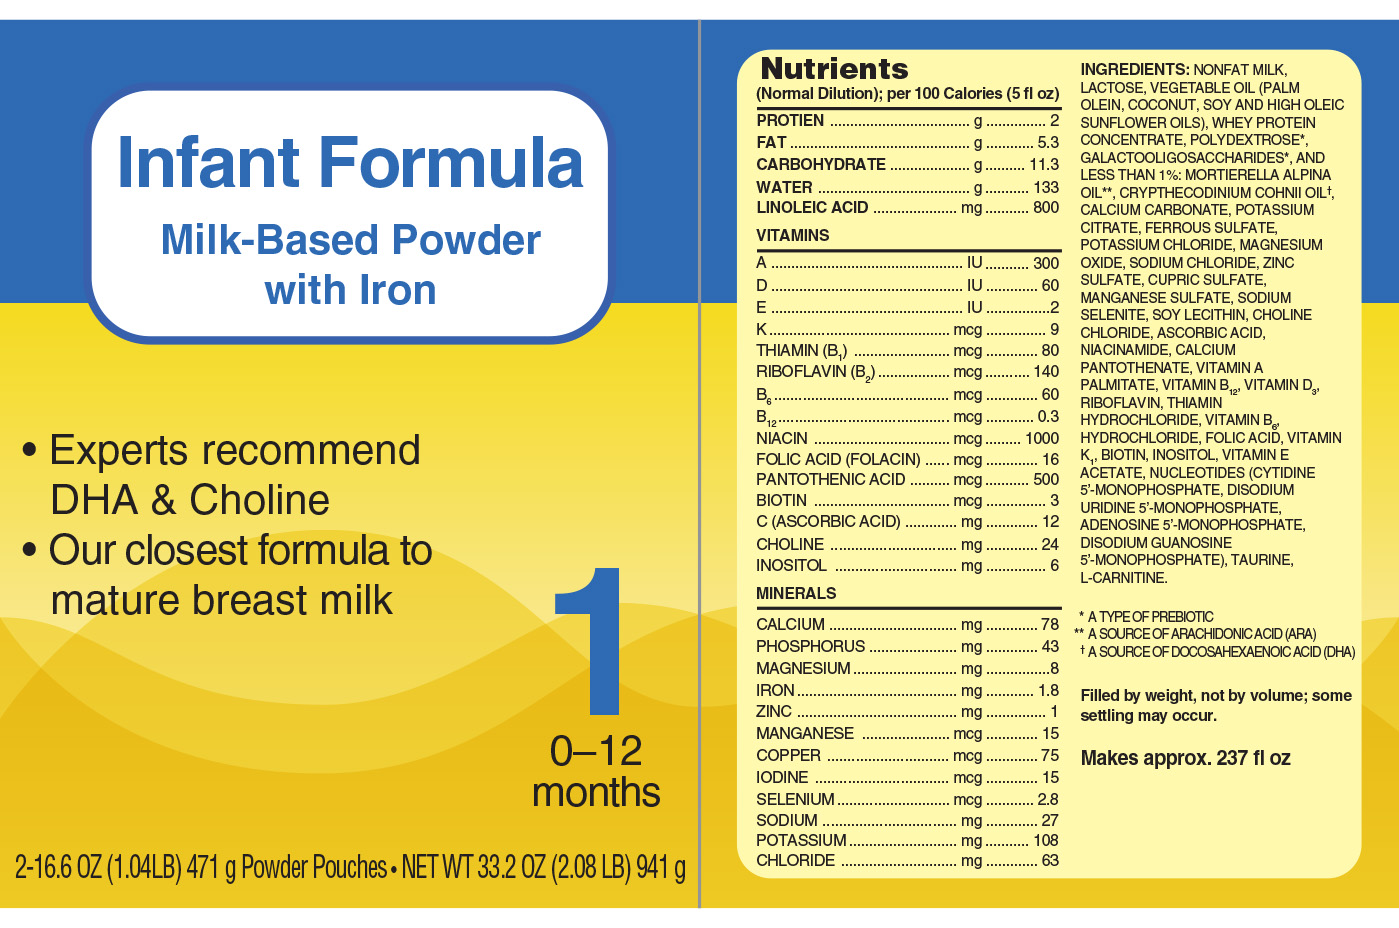
\includegraphics[width=\textwidth]{14_infant_formula_label}
	\caption{Infant Formula Label}
	\label{fig:infant-formula-label}
\end{figure}

\subsection{When to Introduce Solid Food}\label{subsec:when-to-introduce-solid-food}
\begin{itemize}
	\item Introduce solid food at 6 months
	\begin{itemize}
		\item Tongue movement allows swallowing
		\item Muscle development allows infant to sit up
		\item Digestive system and kidneys have matured
		\item Less likely to develop food allergies
		\item Iron-fortified cereals are well tolerated
	\end{itemize}
\end{itemize}

% End When to Introduce Solid Food

\begin{itemize}
	\item Infants should not eat
	\begin{itemize}
		\item Foods they could choke on
		\item Corn syrup or honey
		\item Goat’s milk
		\item Cow’s milk
		\item Too much salt or sugar
	\end{itemize}
	\item Nutrition-related concerns for infants include
	\begin{itemize}
		\item Allergies
		\item Dehydration
		\item Colic
		\item Anemia
		\item Nursing bottle syndrome
		\item Lead poisoning
	\end{itemize}
\end{itemize}

\subsection{Allergies}\label{subsec:allergies}
\begin{itemize}
	\item Solid foods should be introduced one at a time for a week to watch for allergies
	\item Cow’s milk, egg whites, peanuts, and wheat commonly trigger food allergies
\end{itemize}

\subsection{Dehydration}\label{subsec:dehydration}
\begin{itemize}
	\item Extremely dangerous for infants
	\item Caused by diarrhea, vomiting, and inadequate fluid intake
	\item Pediatric electrolyte solution may be used
\end{itemize}

\subsection{Colic}\label{subsec:colic}
\begin{itemize}
	\item Uncontrollable crying that can last for hours
	\item Precise cause is unknown
\end{itemize}

\subsection{Anemia}\label{subsec:anemia}
\begin{itemize}
	\item Infants are born with enough iron for only 6 months
	\item Anemia can develop
	\item Iron-fortified cereal/supplement may be needed
\end{itemize}

\subsection{Nursing bottle syndrome}\label{subsec:nursing-bottle-syndrome}
\begin{itemize}
	\item Leaving an infant alone with a bottle can lead to cavities (dental caries) and tooth decay
	\item The high-carbohydrate fluid provides an optimal food source for bacteria that cause dental caries
	\item Rather than a bottle, begin using a cup by 8 months and no bottle after 18 months
\end{itemize}

\begin{figure}[H]
	\centering
	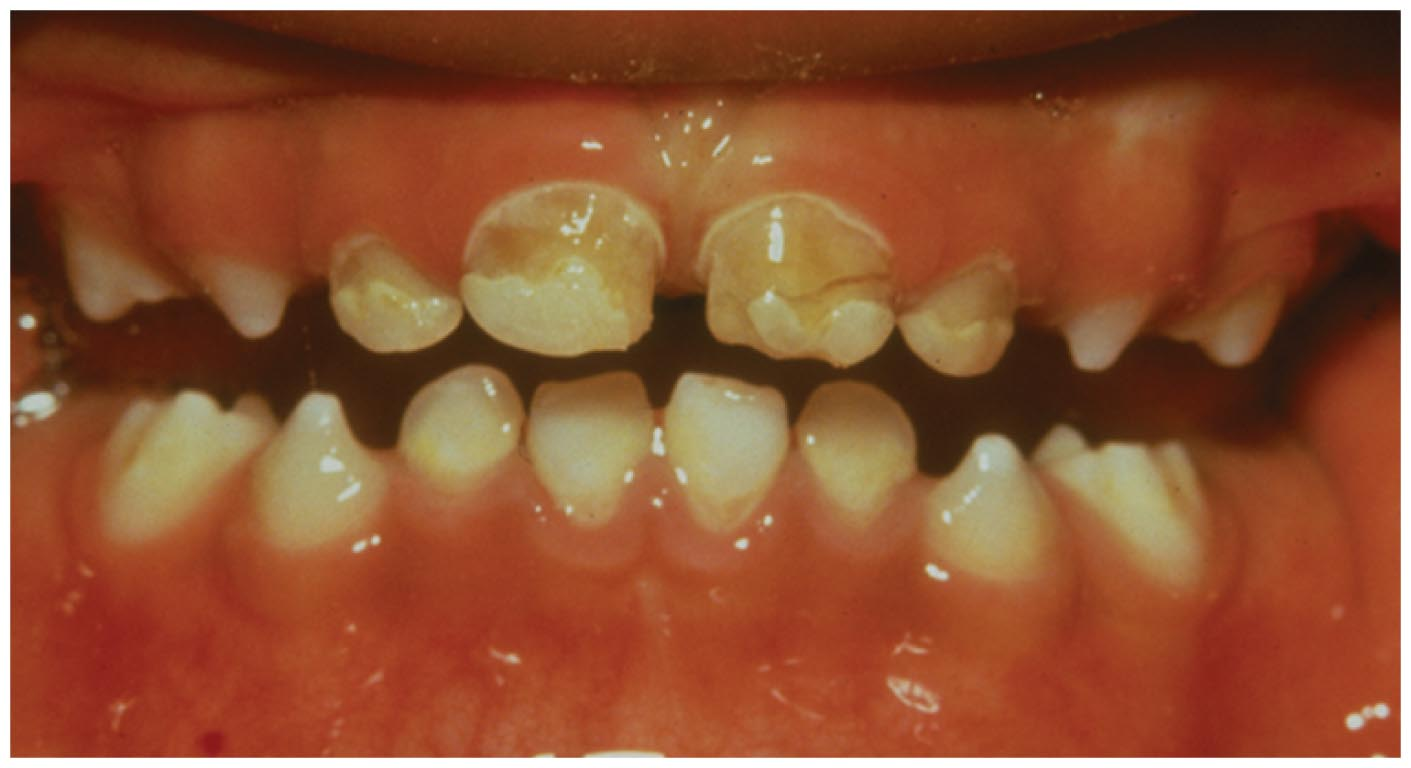
\includegraphics[width=\textwidth]{14_nursing_bottle_syndrome}
	\caption{Nursing Bottle Syndrome}
	\label{fig:nursing-bottle-syndrome}
\end{figure}

\subsection{Lead poisoning}\label{subsec:lead-poisoning}
\begin{itemize}
	\item Especially toxic to infants because the brain and nervous system are still developing
	\item Results in reduced mental capacity, behavioral problems, and impaired growth
	\item Remove old, lead-based paint
	\item Allow tap water to run a minute before use to discard lead leached from pipes
	\item Use only cold tap water because hot tap water is more likely to leach lead
\end{itemize}

\indepth{The Fetal Environment}
\begin{itemize}
	\item Increased evidence suggests that the fetal environment--including a mother’s nutritional status--can influence risks for obesity and chronic diseases later in life
	\item This relationship has been called ``fetal origins theory''
	\item If exposed to famine in the first trimester, the child has increased risk of obesity, coronary heart disease, abnormal serum lipid profile, and metabolic syndrome
	\item \definition{Fetal adaptation}{when a fetus is exposed to harmful elements, it goes into “survival mode”: hormones shift to promote energy storage, and enzymes can increase or decrease the size and function of various body organs}
\end{itemize}

\begin{figure}[H]
	\centering
	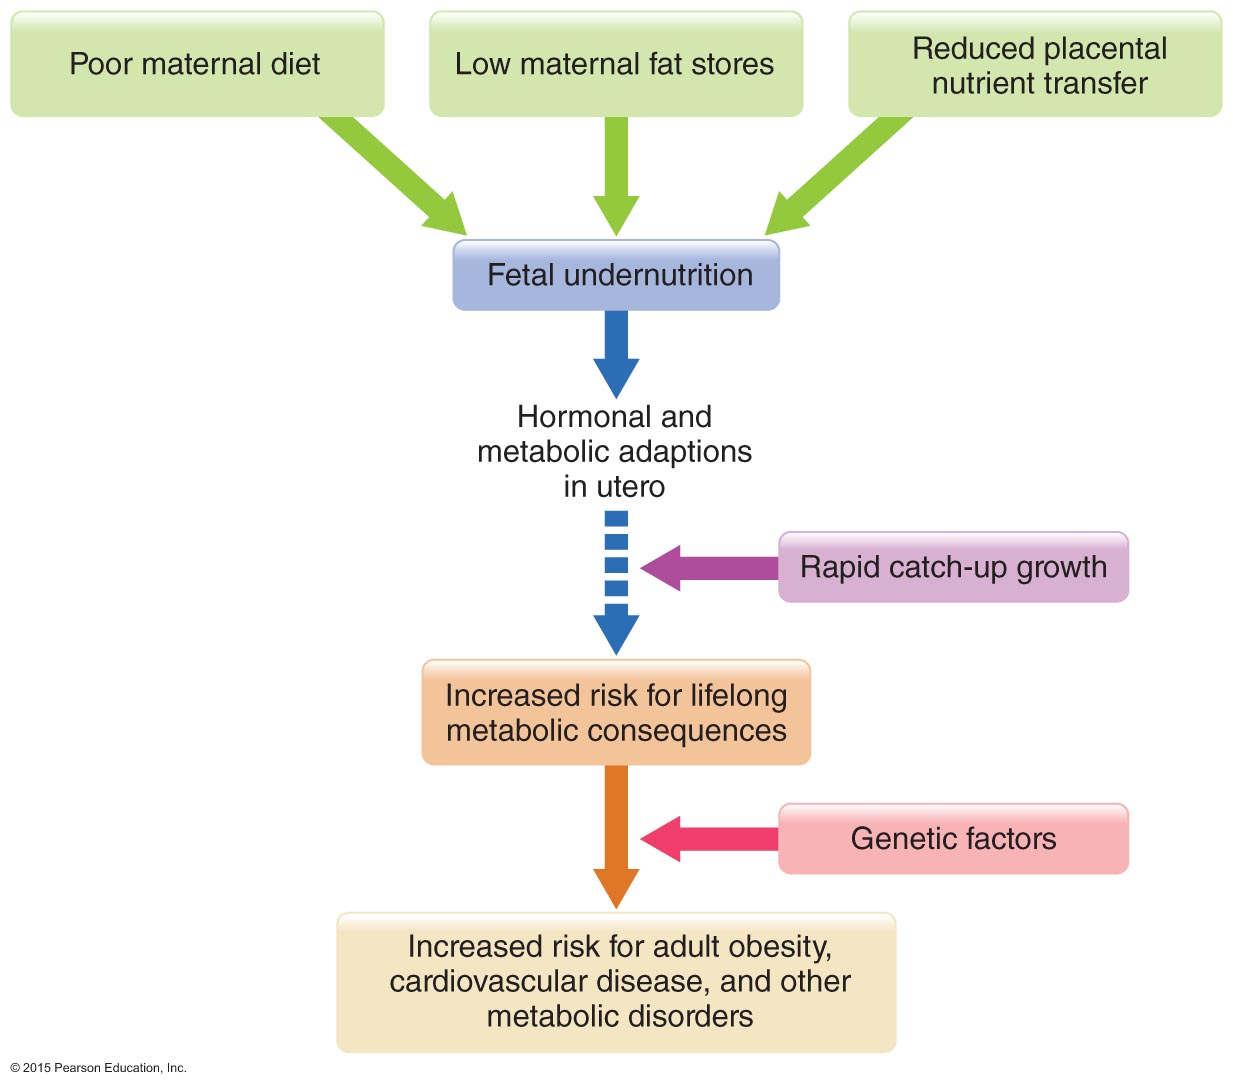
\includegraphics[width=\textwidth]{14_the_fetal_environment}
	\caption{The Fetal Environment}
	\label{fig:the-fetal-environment}
\end{figure}

\begin{itemize}
	\item Fetal stressors that influence adult health include nutrient deficiencies
	\begin{itemize}
		\item Low maternal intake of calcium increases risk of hypertension in offspring
		\item Poor maternal folate intake is linked to neural tube defects and early signs of atherosclerosis
		\item Zinc deficiency has been linked to later-life disorders such as diabetes and atherosclerosis
	\end{itemize}
	\item Strong evidence links maternal dietary excesses to health problems in adult offspring
	\begin{itemize}
		\item Maternal obesity may account for changes in the “programming” of the fetal brain, resulting in lifelong health consequences
		\item Maternal obesity increases rates of spina bifida, neural tube defects, infant heart defects, cleft lip and palate, and abnormal arms or legs
		\item Maternal diabetes can increase risks of infant type 2 diabetes, overweight, and metabolic syndrome
	\end{itemize}
	\item Other detrimental maternal impacts on a fetus include exposure to
	\begin{itemize}
		\item Alcohol
		\item Tobacco
		\item Toxic agents, such as environmental pollutants
	\end{itemize}
\end{itemize}
%</Chapter14>

\end{document}
